\section{Pretrained language models: protocol and complete results}
\label{app:llm-study}

\subsection{Why the additive module is covered by the observation model}

\begin{proposition}[Fixed isometric embedding]
\label{prop:llm-embedding}
Let $E$ be a known linear isometry from the product space
$\RR^{L\times D}$ to a space of layer-weight perturbations, with
$E^*E=I$, and let $W=W_0+E(AB)$ with fixed known $W_0$.
For Euclidean updates of $Z,B$ with the rates and temperature in
Section~\ref{sec:response_identifiability}, the effective weight response
 to a full-space gradient $H$ is
\[
 -\dot W=E\,\mathcal R_{A,B}(E^*H).
\]
Equality of complete full-space response operators is equivalent to
 equality of the factor response operators. Product and response distances
 for embedded observations are unchanged. Consequently the identification
 and stability results apply to this module under their original rank,
 interior, rate, dimension and noise assumptions.
\end{proposition}
\begin{proof}
The derivative of the affine embedding is $E$, so the chain rule pulls
$H$ back to $G=E^*H$. The specified factor updates therefore produce
$-\dot\Theta=\mathcal R_{A,B}(G)$, and differentiation of the embedding
 gives the displayed equation. Conversely, any $G$ is realized by $H=EG$,
 because $E^*EG=G$. Applying $E^*$ to the embedded response recovers
$\mathcal R_{A,B}(G)$, proving both directions of the operator equivalence.
The product coordinates are $E^*(W-W_0)=AB$. Finally,
$\|EX\|_F=\|X\|_F$ preserves all stated product/query/response norms.
The existing identification and stability results therefore apply with
 their original assumptions. Efficient solution of the inverse problem
 remains a separate question.
\end{proof}

Our $E$ inserts 64 evenly spaced output rows into each attention output
projection, leaving the other rows and the pretrained backbone fixed.
All input channels are retained. Thus $D=64d_{\rm in}$, which need not
 equal $64$ times the model's hidden width when attention head dimensions
 differ. The table reports actual projection dimensions. Four FP32 bases
 and FP32 softmax logits are shared over all $L$ matching layers. The
 fixed-row insertion is an isometry in exact arithmetic. Mixed-precision
 backbone execution supplies measured directions; FP64 factor-map auditing
 isolates the mathematical response from rounding in the backbone.
The proposition does not say that natural task gradients realize every
 possible query, nor that nonlinear network-output responses are isometries.

\subsection{Frozen design, data and adaptation}

\paragraph{Model choice and access.}
The nine exact Hugging Face model IDs and revision commits are stored in
\texttt{research/LLM\_ACCESS\_INVENTORY.json}; downloaded snapshot file
 hashes are separately recorded in \texttt{LLM\_MODEL\_BYTES.json}.
Pythia and SmolLM2 use the named base models. Qwen3 uses the named dense
 non-Base releases, so architecture, pretraining and post-training are
 confounded across families. Initial unauthenticated requests for Llama3.2
1B and 3B returned HTTP 401; both are recorded as unavailable, with the
 public SmolLM2 fallback chosen before pilot outcomes. There are no Llama
 results and no coverage of MoE, multimodal models, or models above 8B.

\paragraph{Development and freeze.}
Three representative corrected pilots use Pythia160M, Pythia1B and
Qwen3-0.6B, seed90, 20 updates. Earlier development records retain a
 failed keyword call and an incorrect WikiText article separator; these
 are excluded from the confirmatory evidence. The separator was corrected
 to top-level article headings before the final pilots and all main runs.
The final protocol, 17 source/config/data files and raw corpus hashes were
 frozen before calibration and evaluation. The four calibration units are
Pythia160M and Pythia1B, each seeds101/102. Evaluation uses seeds0/1/2 for
 every model; no checkpoint or seed is selected by validation performance.
Policy thresholds are fixed before evaluation recovery scoring. Evaluation
 gradient collection can run concurrently with calibration because it does
 not inspect recovery quality. The full chronology is retained in
\texttt{research/LLM\_DEVELOPMENT\_LOG.md}.

\paragraph{Data and disjoint roles.}
WikiText-2 train supplies adaptation; validation supplies general-text
 calibration, and test supplies general-text evaluation. GSM8K's public
 training JSONL and MBPP's public JSONL supply held-out math and code text.
Dataset repository commits and raw SHA-256 hashes are in
\texttt{LLM\_CORPUS\_LOCK.json}. This use of public text is not an official
 benchmark-accuracy evaluation. We format math as question plus reference
 answer, and code as comment prompt plus reference program, scoring the
 entire sequence. We do not execute programs or score generated answers.
Public pretraining overlap is unknown.

Within each held-out corpus, alternating documents are assigned to probe
 and loss roles before tokenization. Each role is EOS-concatenated and
 divided into nonoverlapping 129-token blocks (128 prediction targets),
 retaining at most 256 blocks; source document IDs and token hashes are
 stored. Training draws from up to 4,096 train blocks. Twelve distinct
 probe blocks are sampled per checkpoint/domain: the first eight are
 fitting candidates and the last four are reserved for response prediction.
Loss evaluation uses the first 32 loss-role blocks, in 16 batches of two.
The same documents can contribute multiple probe blocks, so query cases
 are not independent statistical replicates. Corpus partition names for
 code/math describe study roles, not official benchmark test splits.

\paragraph{Adaptation budget.}
Each run trains only the $4D+4L$ adapter parameters for 256 updates,
 batch size 4 and sequence length 128, or 131,072 prediction tokens. AdamW uses
 basis learning rate $10^{-3}$ and router rate $10^{-2}$, zero weight decay,
 gradient norm clipping at 1, 16 linear warmup steps, then cosine decay to
0.1 of the initial rate. Initial logits are standard normal, and initial
 bases are nonzero Gaussian matrices scaled by $0.01/\sqrt{d_{\rm in}}$.
The last checkpoint is used. This fixed budget is not a convergence
 certificate or an optimization comparison. Mean router $\ell_1$ movement
 is $0.250$--$0.850$ across checkpoints; minimum router entries are
$6.86\times10^{-4}$--$0.0114$, minimum router singular values
$0.415$--$2.39$, and minimum basis singular values $0.624$--$6.52$.
These are measured properties, not acceptance-policy inputs derived from
hidden truth. Table~\ref{tab:llm-adaptation} includes adverse domain shifts.
The noise grid is not restricted to the global theorem's domain-dependent
 product-noise threshold, and the numerical solver does not enforce its
 entire prescribed domain. Small observed errors therefore do not measure
 the theorem's universal feasible-set diameter or certify its constants.

\begin{table}[t]
\centering\small
\caption{Adapter-induced change in held-out token NLL (adapted minus frozen backbone), averaged over three adapter seeds. Negative is lower. Domains use 32 fixed blocks per checkpoint. Tokenizers differ, so changes are within-model comparisons; these are not answer-accuracy or code-execution scores.}
\label{tab:llm-adaptation}
\begin{tabular}{lrrr}
\toprule
Model & General & Code & Math\\
\midrule
Pythia 160M & -0.0481 & +0.0303 & +0.1146\\
Pythia 1B & -0.4439 & +0.0485 & +0.0812\\
Pythia 2.8B & -0.4220 & +0.0301 & +0.0256\\
Qwen3 0.6B & -0.7086 & -0.0392 & +0.0036\\
Qwen3 1.7B & -0.5666 & -0.1779 & -0.2103\\
Qwen3 4B & -0.6006 & -0.1514 & -0.2646\\
Qwen3 8B & -0.4193 & -0.1729 & -0.2005\\
SmolLM2 360M & -0.3016 & +0.0013 & +0.0216\\
SmolLM2 1.7B & -0.3080 & +0.0071 & +0.0461\\
\bottomrule
\end{tabular}
\end{table}


\subsection{Observations, estimators and transfer diagnostics}

\paragraph{Observation grid and arithmetic.}
Each evaluation checkpoint supplies five families, three query budgets and
 four noise levels: 60 cases, or 1,620 total. Calibration uses only designed,
Gaussian and general-text queries, giving 36 cases per checkpoint and 144
 total. Designed queries are the repeated-complement unit construction;
$q=8$ repeats its four-query cycle. Gaussian and natural queries are
 individually normalized. Designed-query holdouts are independent Gaussian
 directions; the other families use their last four measured directions.
Product and each response receive fixed-relative-Frobenius-norm Gaussian
 perturbations with common random directions across noise levels.
The product row space is recomputed from its noisy observation.

The observation code measures each response by reverse-mode factor
 differentiation and a forward-mode JVP, rather than by the analytic
 response formula. Audit temperature and both Euclidean block rates are
 set to one, independently of the AdamW adaptation learning rates.
All formula checks have relative error at most
$1.62\times10^{-16}$. A common factor permutation preserves the response;
 a fixed non-permutation transform preserves the product to rounding while
 changing the response by $0.103$--$0.481$ on tested directions. This is a
 finite witness, not a test of every alternative. Same-forward-graph chain
 checks pass, but separately repeated BF16 backbone backward passes differ
 by up to $0.0126$ relatively; measured directions are treated as fixed
 inputs afterward. At finite step $10^{-5}$, FP64 response errors are
$1.01\times10^{-9}$--$6.88\times10^{-9}$, versus the much larger FP32/BF16
 errors reported in the main text. These casts are not an experiment on
 mixed-precision optimizer steps with FP32 master weights.

\paragraph{Recovery and scoring.}
The three estimators are spectral recovery, simplex-projected spectral
 recovery with a basis refit, and constrained joint least squares with
 three starts and at most 80 function evaluations per start. All operate
 on compressed observations. Compression retains the product component
 outside the fitted row space and the orthogonal response residual, so an
 estimated-subspace fit cannot silently discard unexplained energy.
Ground truth enters only afterward in the permutation-aligned error
\[
 e=\min_P\left(\frac{\|\widehat A-AP\|_F^2}{\|A\|_F^2}
 +\frac{\|\widehat B-P^TB\|_F^2}{\|B\|_F^2}\right)^{1/2}.
\]
Basis error includes the true basis component outside the estimated
 subspace. No compression failures occur in the main grid. All 540
$q=1$ cases fail the sufficient per-layer query rank and skip joint fitting;
 spectral outputs remain recorded. All 1,080 eligible joint fits return.
Raw/projected spectral methods have 580/531 errors above 0.10 over all
1,620 cases; these counts include their insufficient-query outputs.
The joint-fit median is conditional on the 1,080 returned estimates.

\paragraph{Acceptance and uncertainty.}
The common gate requires positive simplex entries, row-sum error below
$10^{-8}$ and sufficient query rank. Scores are residual-only,
 inverse candidate tangent singular value, and a combined residual,
 conditioning, subspace and competitive-start-disagreement score with a
$10^{-10}$ numerical floor. On calibration, each method/score threshold
 maximizes accepted count subject to at most 5\% bad outputs and at least 20
 accepted cases, keeping ties together; no feasible threshold means all
 reject. Good error is at most 0.05, bad error exceeds 0.10, and intermediate
 cases stay in the denominators. These are empirical policies. Spectral
 estimates often have row-sum errors of order $10^{-8}$--$10^{-7}$ despite
 small factor errors, so their strict gate explains the all-reject policy;
 simplex projection is an explicitly reported separate estimator.

\begin{table}[t]
\centering\small
\caption{Unchanged calibration policies transferred to 1,620 held-out cases per estimator. Coverage includes all 540 insufficient-rank cases at $q=1$; joint fitting is not run there. Bad means permutation-aligned factor error $>0.10$. An empty accepted set has undefined bad fraction. Raw spectral estimates fail the strict simplex gate in calibration, yielding an all-reject policy.}
\label{tab:llm-acceptance}
\begin{tabular}{llrrrr}
\toprule
Estimator & Score & Accepted & Coverage & Bad & Bad / accepted\\
\midrule
Spectral & Residual & 0 & 0.0\% & 0 & --\\
Spectral & Condition & 0 & 0.0\% & 0 & --\\
Spectral & Combined & 0 & 0.0\% & 0 & --\\
Projected & Residual & 1037 & 64.0\% & 20 & 1.93\%\\
Projected & Condition & 960 & 59.3\% & 48 & 5.00\%\\
Projected & Combined & 1056 & 65.2\% & 43 & 4.07\%\\
Joint & Residual & 868 & 53.6\% & 0 & 0.00\%\\
Joint & Condition & 1080 & 66.7\% & 0 & 0.00\%\\
Joint & Combined & 1080 & 66.7\% & 0 & 0.00\%\\
\bottomrule
\end{tabular}
\end{table}


The released summary also includes descriptive intervals from 2,000
 bootstrap resamples of the three adapter checkpoints within each fixed
 model, preserving all query/noise/domain variants within a checkpoint.
They are not population intervals over arbitrary LLMs. In particular,
 resampling zero observed bad joint fits still gives zero; this supplies
 no upper confidence bound on rare or out-of-distribution failures.
Full model/domain breakdowns and all 4,860 method outcomes are retained in
\texttt{results/llm/recovery-cases.csv}.

\subsection{Secondary conditioning stress}

A separate prospectively recorded secondary sweep transforms the learned
Pythia1B, Qwen3-4B and SmolLM2-1.7B factors at seed0. For
$t\in\{1,0.1,0.01,0.001\}$ it either contracts routers toward the uniform
 row (router-rank stress), interpolates toward balanced one-hot rows
 (interior stress), or scales the smallest basis singular value by $t$
 (basis-rank stress). Four designed queries, noise0 or $10^{-4}$, and
 unchanged estimators/policies give 72 cases. These are artificial factor
 modifications, not additionally trained models or real task gradients at
 the modified checkpoint.

\begin{figure}[t]
\centering
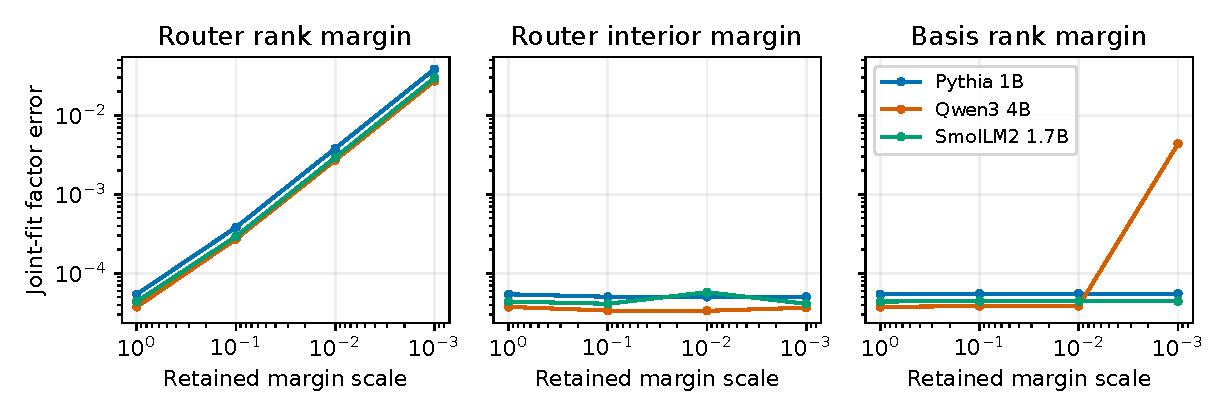
\includegraphics[width=\linewidth]{figures/llm_conditioning.pdf}
\caption{Secondary stress at observation noise $10^{-4}$.
Shrinking router rank amplifies error from roughly $4$--$5\times10^{-5}$
 to $0.027$--$0.038$. The other tested paths do not show comparable
 monotone growth; the absence of failure on a selected path does not
 remove the theorem's nondegeneracy assumptions.}
\label{fig:llm-conditioning}
\end{figure}

\subsection{Matched structural decisions and repeat controls}

The predeclared decision units are Pythia1B, Qwen3-4B and SmolLM2-1.7B,
 each at seeds0/1/2. Every action uses four nonempty equal-sized groups.
The native and recovered router actions maximize balanced assignment
 scores; the effective-parameter control uses balanced $k$-means with
 deterministic farthest-point initialization and 50 iterations; the random
 control uses a fixed seeded balanced partition. Recovered actions use
 general-text $q=4$ joint fits at noise $10^{-4}$ and $10^{-2}$.
Every hard group receives the mean of the same canonical FP32 effective
 tensors, followed by 64 updates of only the four bases with fresh AdamW
 states, rate $10^{-4}$, zero decay, the same batch indices and clipping.
All 45 actions complete. Rejected recovery would retain the native action;
 all 18 recovered decision inputs are accepted by the combined policy.

\begin{table}[t]
\centering\small
\caption{Post-recovery NLL minus native-router partition, averaged over three seeds. All actions use four balanced groups, a common effective-tensor refit and 64 matched updates. Both recovered and effective-clustering partitions equal the native partition at all nine checkpoints. Small Pythia discrepancies under equivalent partitions are numerical execution variation, not structural improvements. Per-seed values and immediate losses are retained in the released CSV.}
\label{tab:llm-decisions}
\begin{tabular}{llrrr}
\toprule
Model & Action & General & Code & Math\\
\midrule
Pythia 1B & Effective clustering & -0.0004 & -0.0005 & -0.0001\\
Pythia 1B & Random balanced & +0.0629 & -0.0196 & -0.0291\\
Pythia 1B & Recovered, $10^{-4}$ & -0.0004 & -0.0005 & -0.0002\\
Pythia 1B & Recovered, $10^{-2}$ & +0.0001 & -0.0007 & -0.0003\\
Qwen3 4B & Effective clustering & +0.0000 & +0.0000 & +0.0000\\
Qwen3 4B & Random balanced & +0.0801 & +0.0096 & +0.0010\\
Qwen3 4B & Recovered, $10^{-4}$ & +0.0000 & +0.0000 & +0.0000\\
Qwen3 4B & Recovered, $10^{-2}$ & +0.0000 & +0.0000 & +0.0000\\
SmolLM2 1.7B & Effective clustering & +0.0000 & +0.0000 & +0.0000\\
SmolLM2 1.7B & Random balanced & +0.1050 & -0.0041 & -0.0238\\
SmolLM2 1.7B & Recovered, $10^{-4}$ & +0.0000 & +0.0000 & +0.0000\\
SmolLM2 1.7B & Recovered, $10^{-2}$ & +0.0000 & +0.0000 & +0.0000\\
\bottomrule
\end{tabular}
\end{table}


All recovered and effective-clustering partitions have zero co-membership
 difference from the native partition. General-text random-minus-native
 post-recovery NLL is $0.0383$--$0.1098$ across the nine checkpoints;
 held-out code and math differences have mixed signs. This establishes no
 advantage over the effective-parameter control. Equivalent partitions on
Pythia exhibit small numerical NLL differences under the original BF16
 execution. A labeled post hoc diagnostic repeats the \emph{identical}
 native action three times per Pythia1B seed with identical tensors,
 labels, batches and optimizer settings. The largest within-seed/domain
 NLL range is $0.00152$, confirming execution variation on the scale of
 these differences. We do not interpret them as structural improvements.
There is no measured compression speedup: the pretrained backbone remains
 stored and executed in full.

\subsection{Compute, replay and artifact scope}

\begin{table}[t]
\centering\small
\caption{Per-checkpoint costs: median over three seeds; maximum allocated GPU memory across training and observation. Training excludes loading, evaluation and gradient collection; observation covers the entire noise/query sweep; recovery is single-thread CPU time elapsed for all three estimators. Timings are local measurements under concurrent jobs.}
\label{tab:llm-cost}
\begin{tabular}{lrrrrrr}
\toprule
Model & Adapter (M) & Train (s) & Observe (s) & Recover (s) & Peak (GiB)\\
\midrule
Pythia 160M & 0.197 & 3.2 & 14.9 & 10.4 & 0.75\\
Pythia 1B & 0.524 & 5.8 & 35.6 & 9.7 & 2.65\\
Pythia 2.8B & 0.655 & 11.8 & 45.3 & 34.4 & 6.68\\
Qwen3 0.6B & 0.524 & 10.4 & 36.3 & 25.3 & 2.82\\
Qwen3 1.7B & 0.524 & 12.4 & 36.1 & 26.7 & 5.26\\
Qwen3 4B & 1.049 & 20.0 & 72.4 & 43.3 & 10.95\\
Qwen3 8B & 1.049 & 34.3 & 72.4 & 43.3 & 19.08\\
SmolLM2 360M & 0.246 & 9.9 & 18.9 & 36.0 & 1.50\\
SmolLM2 1.7B & 0.524 & 9.4 & 35.8 & 19.6 & 4.49\\
\bottomrule
\end{tabular}
\end{table}


The experiments used eight RTX 5090 GPUs with about 32 GiB each. Model
 training ran in a dedicated environment with Transformers 4.57.6 and
PyTorch 2.7.0a0 (NVIDIA build); the previous project environment was retained.
The largest allocated GPU footprint was 19.08 GiB. Per-checkpoint timing
 includes explicit synchronization for training; total training-stage
 timing additionally includes loading, evaluation and natural-gradient
 collection. Recovery is performed on CPU, with up to 12 jobs in parallel.
The complete environment, source freeze, corpus lock, checkpoint hashes,
 observations and per-case solver records are retained.

An isolated PyTorch 2.7.1 CPU environment replays 81 selected cases:
 every evaluation checkpoint, $q=4$, designed/noiseless and general-text
 natural queries at noise $10^{-4}$ and $10^{-2}$. Across 243 estimator
 outputs, the largest permutation-aligned estimate difference is
$1.39\times10^{-10}$, and all acceptance decisions agree. Three additional
 full-dimensional natural-query checks compare explicit analytic residuals
 against the compressed objective for deliberately wrong candidates;
 absolute discrepancies are below $3.8\times10^{-15}$. This is independent
 arithmetic replay, not independent pretrained-model training or external
 peer review. The source package contains the manuscript; the research
 artifact separately contains observations, checkpoints, protocols and
 commands. Upstream model weights and raw gradient caches are not bundled
 with the manuscript. Scripts regenerate them from pinned inputs.
